\documentclass[dvipdfmx]{beamer}
%%%%%%%%%%%%%%%%%%%%%%%%
% Theme
% \usetheme{Singapore}
% \usetheme{Szeged}
% \usetheme{CambridgeUS}
\usetheme{Madrid}
%%%%%%%%%%%%%%%%%%%%%%%%
\useinnertheme{rounded}
%%%%%%%%%%%%%%%%%%%%%%%%
\useoutertheme{infolines}
% \useoutertheme{tree}
%%%%%%%%%%%%%%%%%%%%%%%%
% \usecolortheme[RGB={102,0,204}]{structure}\usecolortheme{dolphin}
% \usecolortheme[RGB={204,0,102}]{structure}\usecolortheme{dolphin}
\usecolortheme[RGB={0,128,0}]{structure}\usecolortheme{dolphin}
% \usecolortheme{fly}
%%%%%%%%%%%%%%%%%%%%%%%%
\setbeamertemplate{navigation symbols}[only frame symbol]{}
%%%%%%%%%%%%%%%%%%%%%%%%
\usepackage[moga-mobo]{pxchfon}
\renewcommand{\kanjifamilydefault}{\gtdefault}
\hypersetup{colorlinks,linkcolor=,urlcolor=blue}
\usepackage{bxdpx-beamer}
\usepackage{atbegshi}
\ifnum 42146=\euc"A4A2 \AtBeginShipoutFirst{\special{pdf:tounicode EUC-UCS2}}\else
\AtBeginShipoutFirst{\special{pdf:tounicode 90ms-RKSJ-UCS2}}\fi
\usepackage{amsmath}
\usepackage{dialogue}
\title{\TeX による不動産投資シミュレーション}
\author{tattsan}
\date{}
\newcommand{\たつ}{たつ}
\begin{document}
%%%%%%%%%%%%%%%%%%%%%%%%%%%%%%%%%%%%%%%%%%%%%%%%%%%%%%%%%%%%%%%%%%
\begin{frame}\frametitle{}
\maketitle
% \titlepage %表紙
\onslide<2->{なんでソレをアレで}
\end{frame}
% \def\thesection{第\xkansuji{section}話}
% \setcounter{section}{\xintiSub{\xintiPow{2}{31}}{4}}%% 2^{31}-4

\section{ほげ} 

\begin{frame}[fragile]\frametitle{動機}
  不動産で成功すると\alert{大統領になれる}ことがわかったので、
  自分も不動産に投資することにした。
  そこそこ勉強したのち業者を訪ねて実情を尋ねてみたら、
  資料の中にシミュレーションと称するデータがあった。
\begin{block}{}\small
  \begin{dialogue}
    \speak{\たつ} \onslide<2->{これは一体どういう計算をしているのですか?}
    \speak{業者}  \onslide<3->{それは大変難解な数式を用いるものでして…}
  \end{dialogue}
\end{block}
\onslide<4->{%
  数学教師に「数式が難解である」と主張するくらいだから、
  それはよほど難解なのだろう。自宅に戻って自分で計算してみることにした。
  }
\end{frame}


\begin{frame}[fragile]\frametitle{アプリケーションの選択}
  さて計算には何を使用すればよいだろうか。
  最近本業でお世話になっているのはPGFである。
  だが仮に投資が成功して莫大な金額を扱うようになると、
  PGFでは\alert{桁数が足りないかも}知れない。
  そこで3年前に
  \href{https://adventar.org/calendars/553}{\TeX ~\& \LaTeX ~Advent Calendar 2014} の
  \href{https://github.com/tattsan/xkansuji/wiki/texadventar14}{10日目の記事}で紹介した
  \alert{\textsf{xintパッケージ}}
  を利用することにした。
\end{frame}

\begin{frame}[fragile]\frametitle{アプリケーションの熟慮}
  いやしかしこれはおかしい。比較したのは\TeX のライブラリだけであり、\TeX 以外の選択肢を考えていないではないか?
  \bigskip\par
  \onslide<2->{{\Large しかし 2015年, 2016年 と2年の長きにわたって自分は \TeX ~\& \LaTeX ~Advent Calendar に参加していないでいる。}}
  \bigskip\par
  \onslide<3->{選択の余地は無かった。}
\end{frame}

\begin{frame}[fragile]\frametitle{シミュレーションの概要}
  考慮すべき事柄は次のようなものだ。
  \begin{block}{}\small
    \begin{itemize}
    \item 物件価格と$\text{[利回り]}=\dfrac{\text{想定年間家賃収入}}{\text{物件価格}}$
    \item 自己資金・融資金額・融資金利・返済期間
    \item 購入時諸経費・運営時諸経費・売却時諸経費
    \item 空室・家賃の下落・売却価格の減衰などの劣化因子
    \end{itemize}  
  \end{block}
  シミュレーションが必要になる最大の要因はローンの返済にある。
  この返済のために、空室などの収入低下があると一気に経営が厳しくなる。
  業者の見せる夢のようなシミュレーション結果など信じてはいけない。
\end{frame}

\begin{frame}[fragile]\frametitle{私家版\textsf{tsfudosan}パッケージ}
  それで作成した\LaTeX マクロ集が「私家版\textsf{tsfudosan}パッケージ」である。
  「私家版」の接頭語ははずせない。
  それは汎用パッケージが満たすべき作法を一切守っていない。
  コードの書き方も滅茶苦茶で、ともかく目の前にシミュレーション結果が出ることを
  最優先して書き散らしたものである。
  \begin{block}{}\small
    \begin{itemize}
    \item 名前の衝突を避ける命名法はしていない。
    \item ユーザコマンドと内部コマンドの区別が付いてない。
    \item 局所変数にしていたハズのものを都合によりグローバルに値を変更し、
      抜けるときに戻せばいいや、とは思っただけでそのまま放置
    \end{itemize}  
  \end{block}
  など見るに耐えないものになっている。だからこのスライドも2014年のスライドと同様、
  \alert{\textsf{xintパッケージ}}の使い方の紹介でしかない。
\end{frame}

\begin{frame}[fragile]\frametitle{入力例}
\begin{block}{}\tiny
\begin{verbatim}
\documentclass[platex,a4paper,base=8.4pt,nomag,landscape,dvipdfmx]{bxjsarticle}
\setpagelayout{left=10mm,right=10mm,top=5mm,bottom=5mm,headsep=0mm,footskip=0mm}
\usepackage{tsfudosan}
\begin{document}
%%%%%%%%%%%%%%%%%%%%%%%%%%%%%%%%%%%%%%%%%%
\def\初年号{17}% 初年度の西暦下二桁
\def\年表示{$\arabic{経過年数}\equiv 20\動年号$}
%%%%%%%%%%%%%%%%%%%%%%%%%%%%%%%%%%%%%%%%%%
% 物件関連
\def\物件名{ほげ荘}%
\def\物件価格{8000.0000}%
\def\物件購入手数料率{0.07}%
%%%%%%%%%%%%%%%%%%%%%%%%%%%%%%%%%%%%%%%%%%
% 融資関連
\def\頭金率{0.3}%
\def\融資返済年数{25}%
\def\繰上返済手数料率{0.02}%
\def\融資金利{0.018}%
%%%%%%%%%%%%%%%%%%%%%%%%%%%%%%%%%%%%%%%%%%
% 運営関連
\def\運営費率{0.15}%
\def\初年想定総収入{608.0000}%
\def\空室率{0.15}%
\def\家賃減衰率{0.015}%1年あたり
\def\売却価格減衰率{0.02}%1年あたり
%%%%%%%%%%%%%%%%%%%%%%%%%%%%%%%%%%%%%%%%%% 
\def\物件サブタイトル{:最初の例}%
\MakeSheet
\end{document}
\end{verbatim}
\end{block}
\end{frame}

\begin{frame}[fragile]\frametitle{出力結果}
  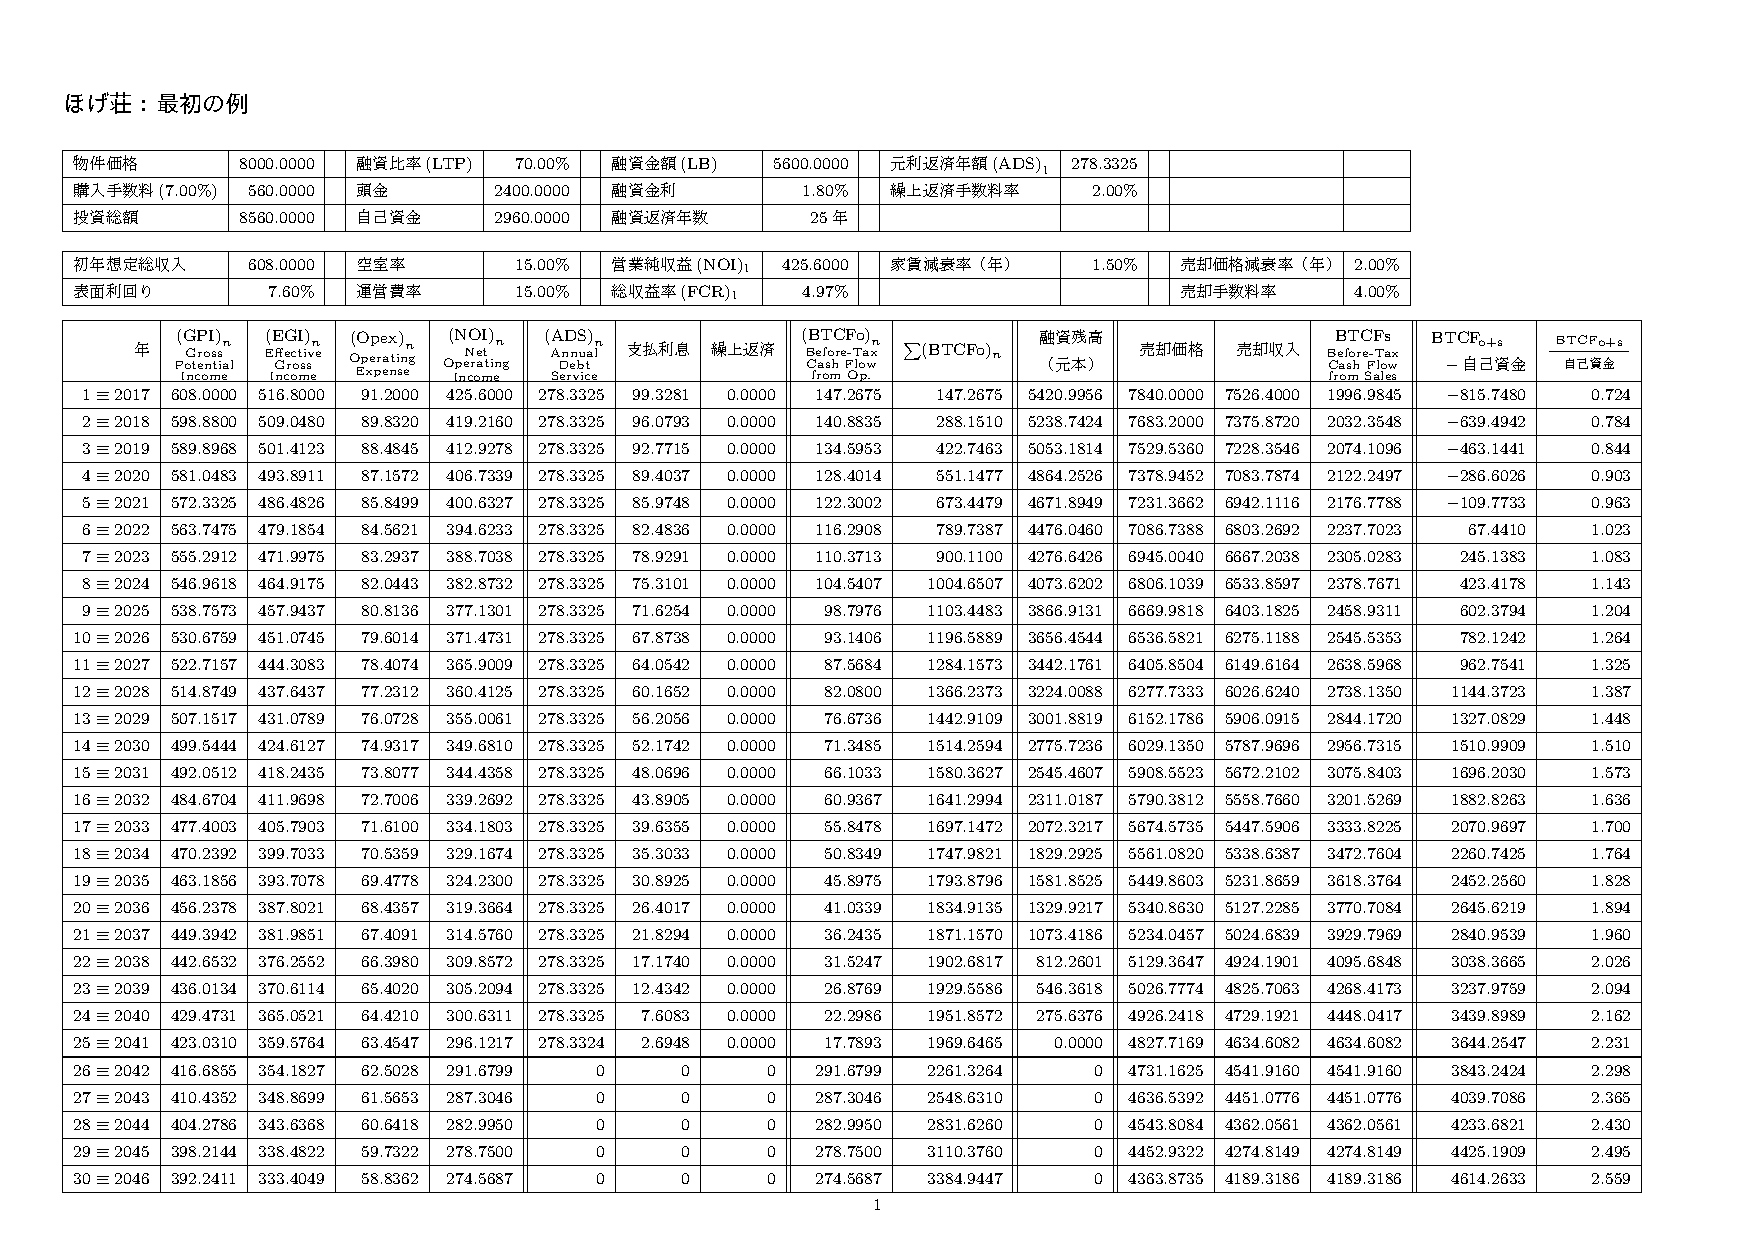
\includegraphics[page=1,width=1.05\textwidth,keepaspectratio,trim=10 0 0 40]{texdefudosan-demo}
\end{frame}

\begin{frame}[fragile]\frametitle{表の説明}
  単位は万円で小数点以下はそれ未満。表に現れる項目を左から説明する。
  \begin{block}{}\footnotesize
    \begin{itemize}
    \item $(\text{GPI})_n$:満室時の想定賃料収入。家賃減衰率にもとづき減衰する。
    \item $(\text{EPI})_n$:実効的想定賃料収入。空室率によりGPIよりも少ない。
    \item $(\text{Opex})_n$:運営費。EPIに運営費率を乗じたもの。
    \item $(\text{NOI})_n$:純収益。$(\text{EPI})_n-(\text{Opex})_n$の値。
    \item $(\text{ADS})_n$:ローンの元利返済額。金利一定で繰上返済しなければ一定。
    \item 支払利息:$(\text{ADS})_n$のうちの利息返済分。
    \item $(\text{BTCFo})_n$:税引き前キャッシュフロー。$(\text{NOI})_n-(\text{ADS})_n$の値。
    \item $\sum(\text{BTCFo})_n$:$(\text{BTCFo})_n$の積算額。
    \item 売却価格:売却価格減衰率にもとづいて評価した売却価格。
    \item 売却収入:売却価格から諸経費を除いた値。ローン返済前。
    \item $(\text{BTCFs})$:税引き前キャッシュフロー。ローン返済後の収入。
    \end{itemize}  
  \end{block}
  最後の2つの欄は、総収入と最初の資金との対比。完済する25年の所に太線が引かれている。
\end{frame}


\begin{frame}[fragile]\frametitle{ステージの導入と繰上返済(入力)}
  さて若い投資家であればこの収入を次の投資に回すべきであるが、
  年を食ってからスタートした自分としては、働けるうちに将来の不安因子を
  消しておきたい。そこで余裕があれば繰上返済することを考える。
  本業在職中を「ステージA」、退職後を「ステージB」として
  ステージAでは毎年120万円を繰上返済する。この「ステージ」は
  A,B,Cの3つを定義できるようになっている。
  \begin{block}{}\scriptsize
\begin{verbatim}
%%%%%%%%%%%%%%%%%%%%%%%%%%%%%%%%%%%%%%%%%%
\def\物件サブタイトル{:ステージを定義し、繰上返済(定額)を計画}%
\def\退職まで年数{20}%
\def\ABthreshold{\退職まで年数}% 本業在職ステージAと本業退職後のステージBを定義。
\def\BCthreshold{\シミュレーション年数}% Cは定義せず最後までBとする。
\def\繰上返済年額A{120.0000}% 現役の間は、毎年120万を繰上返済。
\def\繰上返済年額B{0.0000}%
\MakeSheet
%%%%%%%%%%%%%%%%%%%%%%%%%%%%%%%%%%%%%%%%%%
\end{verbatim}
  \end{block}
  退職まで年数は実際の私のものではない。
\end{frame}

\begin{frame}[fragile]\frametitle{ステージの導入と繰上返済(出力)}
  \includegraphics[page=2,width=1.05\textwidth,keepaspectratio,trim=10 0 0 40]{texdefudosan-demo}
\end{frame}


\begin{frame}[fragile]\frametitle{動的な繰上返済(入力)}
  さて繰上返済をすると、 $(\text{ADS})_n$ が減ってくれるので余裕が生まれる。
  その分も繰上返済に回すという、動的な返済計画が可能である。
  \begin{block}{}\tiny
\begin{verbatim}
%%%%%%%%%%%%%%%%%%%%%%%%%%%%%%%%%%%%%%%%%%
\def\物件サブタイトル{:動的な繰上返済}%
\def\繰上返済年額A{\xintRound{4}{
  \xintifboolexpr{\the経過年数 = 1}{0.0000}{
     \xinttheexpr  (max(0, \NOI -20.0000 - \修正年間元利金返済))/(1+\繰上返済手数料率) \relax
}}}%
\def\繰上返済年額B{\xintRound{4}{
  \xinttheexpr  (max(0, \NOI -200.0000 - \修正年間元利金返済))/(1+\繰上返済手数料率) \relax
}}%
\MakeSheet
%%%%%%%%%%%%%%%%%%%%%%%%%%%%%%%%%%%%%%%%%%
\end{verbatim}
  \end{block}
  ここで\alert{\textsf{xintパッケージ}}が活躍する。
  \begin{itemize}
  \item \verb+\xintifboolexpr+ は条件分岐。初年度は繰上返済しない設定。
    初年度は\alert{不動産取得税}という多額の経費が生じる。
  \item \verb+\xinttheexpr+ は色々な計算式を処理してくれる。繰上返済しなければ
    「\verb+\NOI - \修正年間元利金返済+ 」が税引き前キャッシュフローとなる。
    ステージAでは、それから20万円を差し引いて残りを繰上返済に回している。
  \end{itemize}

\end{frame}

\begin{frame}[fragile]\frametitle{動的な繰上返済(出力)}
  \includegraphics[page=3,width=1.05\textwidth,keepaspectratio,trim=10 0 0 40]{texdefudosan-demo}
\end{frame}

\begin{frame}[fragile]\frametitle{デッドクロス}
  おお退職年にピッタリ返済が完了している、夢のようだ!
  しかし忘れていることがある。それは\alert{税金}だ。
  ローン返済のうち経費として課税対象外となるのは「利息部分のうちの更に建物相当分」のみ。
  つまりローン返済分の大部分は課税対象なので、実際には収入になっていないのに税金を支払わねばならない。
  \bigskip\par
  \onslide<2->{これを大幅に軽減してくれるのが\alert{減価償却費用}だ。
  建物の劣化は、税務上は費用の一種と看倣し、課税対象額から控除される。}
    \bigskip\par
  \onslide<3->{問題は減価償却の可能な期間が決まっていること。期間が過ぎるとその年から突然税金が増える。
  これを\alert{デッドクロス}と呼ぶ。}
\end{frame}

\begin{frame}[fragile]\frametitle{デッドクロスを考慮した繰上返済(入力)}
  ではデッドクロスを考慮した繰上返済の様子を見てみる。
  中古物件では償却期間が短い。それは1年あたりの控除額が大きくなる反面、
  デッドクロスがすぐにやってくるということでもある。
  \begin{block}{}\tiny
\begin{verbatim}
%%%%%%%%%%%%%%%%%%%%%%%%%%%%%%%%%%%%%%%%%%
\def\減価償却期間{10}% 減価償却期間は本業在職中に終わるとする。
\def\ABthreshold{\減価償却期間}% ステージAは減価償却期間とし、
\def\BCthreshold{\退職まで年数}% 退職後のステージをCに変更する。
\def\建物価額{3000}%
\edef\減価償却費{\xintRound{4}{\xinttheexpr \建物価額 /\減価償却期間 \relax}}%
\def\所得税率{0.20}%
\edef\減価償却節税額{\xintRound{4}{\xinttheexpr \減価償却費 *\所得税率 \relax}}%
\def\繰上返済年額A{\xintRound{4}{
  \xintifboolexpr{\the経過年数 = 1}{0.0000}{
     \xinttheexpr  (max(0, \NOI -20.0000 - \修正年間元利金返済))/(1+\繰上返済手数料率) \relax
}}}%
\def\繰上返済年額B{\xintRound{4}{
  \xinttheexpr (max(0, \NOI  -20.0000 - \減価償却節税額 - \修正年間元利金返済))/(1+\繰上返済手数料率) \relax
}}%
\def\繰上返済年額C{\xintRound{4}{
  \xinttheexpr (max(0, \NOI -200.0000 - \減価償却節税額 - \修正年間元利金返済))/(1+\繰上返済手数料率) \relax
}}%
\def\物件サブタイトル{:減価償却と税金を考慮した動的な繰上返済}%
\MakeSheet
%%%%%%%%%%%%%%%%%%%%%%%%%%%%%%%%%%%%%%%%%%
\end{verbatim}
  \end{block}

\end{frame}


\begin{frame}[fragile]\frametitle{デッドクロスを考慮した繰上返済(出力)}
  \includegraphics[page=4,width=1.05\textwidth,keepaspectratio,trim=10 0 0 40]{texdefudosan-demo}
\end{frame}


\begin{frame}[fragile]\frametitle{不動産投資の現実}
  11年目から $(\text{BTCFo})_n$ が60万円増加しているが、これはこの分を税金の支払いに回す必要があると
  いうことだ。退職時に完済と思っていたら、まだ400万円以上の借金が残っていることになる。
    \bigskip\par
    \onslide<2->{
      さて現実には負の因子がたくさんある。
    }
    \bigskip
  \begin{itemize}
  \item \onslide<3->{
      運営費の15\% は最初の業者のシミュレーションから決めたが、
      実際にはもっとイレギュラーな支出があり、15\%では済まないらしい。}
  \item \onslide<4->{
      賃貸住宅は供給過剰なので十分な対策を取らないと空室率が上がる。}
  \item \onslide<5->{
      この2〜3年は不動産バブルで物件価格が高く、マトモにペイする物件は
      流通していない。}
  \item \onslide<6->{
      逆に売却時には不動産バブルがはじけているであろう。}
  \end{itemize}
  \bigskip
  \onslide<7->{
    だがこれらを詳しく議論する事は \TeX とは関係がないのでやめておく。
    }
\end{frame}

  


\begin{frame}[fragile]\frametitle{\TeX の現実}
  このようなシミュレーションを不動産業者に見せた所、彼はこう言った。
  \onslide<2->{
  \begin{block}{}\large
    \begin{dialogue}
    \speak{業者} \onslide<2->{これは分りやすいですね。}
    \onslide<3->{プロユースに十分使えます。}
    \onslide<4->{私も是非その}
    \onslide<6->{\alert{Excel}}
    \onslide<5->{マクロを使いたいです。}
    \bigskip
    \speak{\たつ}
    \onslide<7->{\alert{\huge (ちがう!ちがう!ちがう!)}}
    \end{dialogue}
  \end{block}
  }
\end{frame}

\begin{frame}\frametitle{}
  \begin{block}{}\Huge
    \centering おしまい
  \end{block}
\end{frame}

\end{document}

%%% Local Variables: 
%%% mode: japanese-latex
%%% TeX-master: t
%%% End: 
